\chapter{Свёртки за пределами изображений}
\label{chap:convolutions_beyond_images}

\begin{supportbox}{Об этой главе}
Свёрточные модели являются мощной базовой моделью во многих приложениях, выходящих далеко за рамки классификации изображений. В этой главе мы предоставляем обзор нескольких таких расширений, включая использование свёрточных слоев для 1D и 3D данных, моделирование текста и авторегрессионную генерацию. Некоторые из вводимых нами понятий (например, маскирование, токенизация) являются фундаментальными для остальной части книги.
\end{supportbox}

\section{Свёртки для 1D и 3D данных}
\subsection{За пределами изображений: временные ряды, аудио, видео, текст}

В предыдущей главе мы сосредоточились исключительно на изображениях. Однако многие другие типы данных имеют схожие характеристики, т.е. одно или несколько «упорядоченных» измерений, представляющих время или пространство, и одно измерение, представляющее признаки (каналы в случае изображений). Давайте рассмотрим несколько примеров:
%
\begin{enumerate}
\item \textbf{Временные ряды} — это наборы измерений одного или нескольких процессов (например, цены на акции, значения датчиков, потоки энергии). Мы можем представить временной ряд в виде матрицы $\mathbf{X} \sim (t,c)$, где $t$ — длина временного ряда, а $\mathbf{X}_i \sim (c)$ — это $c$ измерений в момент времени $t$ (например, $c$ датчиков с ЭЭГ-сканирования или $c$ цен на акции). Каждый момент времени эквивалентен пикселю, а каждое измерение — каналу.
\item \textbf{Аудио} файлы (речь, музыка) также можно описать матрицей $\mathbf{X} \sim (t,c)$, где $t$ — это теперь длина аудиосигнала, а $c$ — каналы записи ($1$ для монофонического аудио, $2$ для стереосигнала и т.д.). 
%
\begin{supportbox}{Частотный анализ}
    Аудио также можно преобразовать в формат, подобный изображению, с помощью частотного анализа (например, извлекая коэффициенты MFCC по небольшим окнам), и в этом случае результирующие \textit{временно-частотные} изображения представляют эволюцию частотного содержания по сигналу - см. Рисунок \ref{fig:audio_analysis_frequency} для примера. С этой предварительной обработкой мы можем использовать стандартные свёрточные модели для их обработки.
\end{supportbox}
    %
    \item \textbf{Видео} можно описать тензором 4-го ранга $X \sim (t, h, w, c)$, где $t$ — количество \textit{кадров} видео, а каждый кадр — это изображение формы $(h,w,c)$. Другим примером является объемное сканирование в медицине, и в этом случае $t$ — это глубина объема.
\end{enumerate}

\begin{figure}
    \centering
    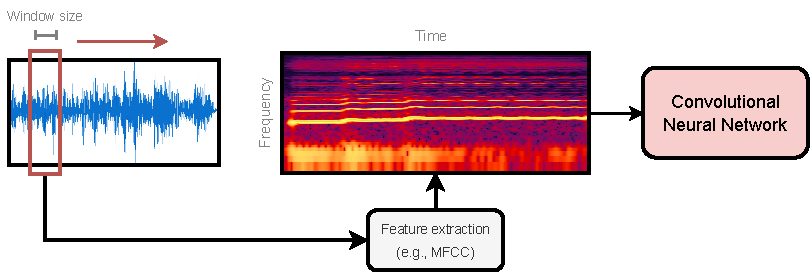
\includegraphics[width=1.0\textwidth]{images/audio_classification_CNN}
    \caption{Аудио можно представить либо как 1D-последовательность (слева), либо как 2D-изображение во временно-частотной области (в центре). Во втором случае мы можем применять те же методы, что и в предыдущей главе.}
    \label{fig:audio_analysis_frequency}
\end{figure}

Временные ряды, аудиосигналы и видео можно описать их \textbf{частотой дискретизации}, которая обозначает, сколько выборок приобретается за единицу времени, иногда выражаемую в выборках в секунду или герцах (Гц). Например, классические ЭЭГ-устройства получают сигналы с частотой 240 Гц, что означает 240 выборок в секунду. Акцию можно проверять каждую минуту, что соответствует 1/60 Гц. Напротив, аудио приобретается с очень высокой частотой для обеспечения точности: например, музыку можно приобретать с частотой $44.1e^3$ Гц (или $44.1$ кГц). Типичные \textbf{частоты кадров} для видео, напротив, составляют около $24$ кадров в секунду (fps), чтобы обеспечить плавность для человеческого глаза.

Разрешение изображения, частота дискретизации аудио и частота кадров видео играют схожие роли в определении точности, с которой приобретается сигнал. Для изображения мы можем априори предположить фиксированное разрешение (например, $1024 \times 1024$ пикселей). Это разумно, поскольку изображения всегда можно изменить до заданного разрешения, сохраняя при этом достаточную согласованность, за исключением очень малых разрешений. Напротив, продолжительность аудио и видео может варьироваться от входа к входу (например, песня продолжительностью 30 секунд против песни продолжительностью 5 минут), и их нельзя изменить до общего размера, что означает, что наши наборы данных будут состоять из данных \textbf{переменной длины}. Кроме того, разрешение аудио может легко стать очень большим: при частоте дискретизации $44.1$ кГц 3-минутное аудио будет иметь $\approx 8$ млн выборок.

Мы также отмечаем, что измерения в этих примерах можно грубо разделить на «пространственные измерения» (например, изображения) или «временные измерения» (например, разрешение аудио). В то время как изображения можно считать симметричными по своим пространственным осям (во многих случаях изображение, перевернутое по ширине, является другим допустимым изображением), время \textit{асимметрично}: аудиосэмпл, инвертированный по своей временной оси, в общем случае недействителен, а инвертированный временной ряд представляет собой ряд, развивающийся из будущего в прошлое. Помимо использования этого аспекта при проектировании наших моделей (\textbf{причинность}), мы также можем быть заинтересованы в \textit{предсказании} будущих значений сигнала: это называется \textbf{прогнозированием}.

Наконец, рассмотрим текстовое предложение, такое как «\textit{кошка сидит на столе}». Существует много способов разбить это предложение на части. Например, мы можем рассмотреть его отдельные слоги: [«\textit{кош}», «\textit{ка}», «\textit{си}», «\textit{дит}», «\textit{на}», «\textit{сто}», «\textit{ле}»]. Это еще один пример последовательности, за исключением того, что каждый элемент последовательности теперь является категориальным значением (слогом), а не числовым кодированием. Следовательно, нам нужен какой-то способ кодирования этих значений в признаки, которые могут быть обработаны моделью: разбиение текстовой последовательности на компоненты называется \textbf{токенизацией}, а превращение каждого токена в вектор — \textbf{вложением} токенов.

В следующих разделах мы рассмотрим все эти аспекты (входы переменной длины, причинность, прогнозирование, токенизация и вложение) по очереди, чтобы увидеть, как мы можем строить свёрточные модели для их решения. Некоторые из вводимых нами техник, такие как маскирование, очень общие и полезны также для других типов моделей, таких как трансформеры. Другие техники, такие как расширенные свёртки, напротив, специфичны для свёрточных моделей.

\subsection{1D и 3D свёрточные слои}

Давайте рассмотрим, как определить свёртки для 1D-сигналов (например, временных рядов, аудио) и их расширение на 3D-сигналы (например, видео). Обратите внимание, что размерность относится только к количеству измерений, по которым мы сворачиваем (пространственным или временным), и не включает измерение канала. Напомним, что в 1D-случае мы можем представить вход в виде одной матрицы:

\vspace{1em}
\begin{equation*}
\mathbf{X} \sim (\eqnmarkbox[drawred]{node}{t}, \eqnmarkbox[drawgreen]{node2}{c})
\end{equation*}
\annotate[yshift=-1em]{below,left}{node}{Длина последовательности}
\annotate[yshift=-1em]{below,right}{node2}{Признаки}

\vspace{1em}
Теперь мы воспроизводим вывод из Главы \ref{chap:cnns}. Для размера патча $s=2k+1$ мы определяем $P_{k}(i) \sim (s,c)$ как подмножество строк в $\mathbf{X}$ на расстоянии не более $k$ от $i$ (игнорируя граничные элементы, для которых можно использовать дополнение нулями). 1D-свёрточный слой $\mathbf{H} = \text{Conv1D}(\mathbf{X})$ выводит матрицу $\mathbf{H} \sim (t, c^\prime)$, где $c^\prime$ — гиперпараметр, определяющий выходную размерность, определяемую построчно как:
%
\begin{equation}
\idx{\text{Conv1D}(X)}{i} = \phi(\mathbf{W} \cdot\text{vect}(P_{k}(i)) + \mathbf{b})
\label{eq:1d_convolution}
\end{equation}
%
с обучаемыми параметрами $\mathbf{W} \sim (c^\prime,sc)$ и $\mathbf{b} \sim (c^\prime)$. Как и в 2D-случае, этот слой является локальным (для правильно измененного определения локальности) и эквивариантным к трансляциям последовательности. 

В 2D-случае мы также обсуждали альтернативную нотацию со всеми индексами, явно суммируемыми:
%
\begin{equation}
H_{ijz} = \sum_{i^\prime=1}^{2k+1}\sum_{j^\prime = 1}^{2k+1}\sum_{d=1}^{c} \idx{W}{i^\prime, j^\prime,z,d}\idx{X}{i^\prime+t(i),j^\prime+t(j),d}
\label{eq:conv_again}
\end{equation}
%
где $t(i)=i+k-1$, как в \eqref{eq:convolutive_offset}. Напомним, что мы используем $t$ для индексации $i^\prime$ и $j^\prime$ по-разному для двух тензоров: от $1$ до $2k+1$ для $W$ и от $i-k$ до $i+k$ для $X$. Эквивалентный вариант для \eqref{eq:1d_convolution} получается тривиально путем удаления одного индекса суммирования:

\begin{equation}
H_{iz} = \sum_{i^\prime=1}^{2k+1}  \sum_{d=1}^{c} \idx{W}{i^\prime,z,d}\idx{X}{i^\prime+t(i),d}
\label{eq:1d_convolution_sum}
\end{equation}

где параметры $W \sim (s, c^\prime, c)$ теперь организованы в тензор 3-го ранга. Напротив, 3D-вариант получается путем добавления нового суммирования по третьему измерению с индексом $p$:

$$
H_{{\color{drawred}p}ijz} = {\color{drawred}\sum_{p^\prime=1}^{2k+1}}\sum_{i^\prime=1}^{2k+1}\sum_{j^\prime = 1}^{2k+1},\sum_{d=1}^{c} \idx{W}{{\color{drawred}p^\prime}, i^\prime, j^\prime,z,d}\idx{X}{{\color{drawred}p^\prime+t(p)},i^\prime+t(i),j^\prime+t(j),d}
$$

Мы предполагаем, что размер ядра одинаков по всем измерениям для простоты. С аналогичными рассуждениями мы можем вывести векторизованный 3D-вариант свёртки, а также 1D и 3D варианты макс-пулинга.


\section{Свёрточные модели для 1D и 3D данных}

Теперь мы рассмотрим проектирование свёрточных моделей в 1D-случае, с акцентом на то, как обрабатывать входы переменной длины и как работать с текстовыми последовательностями. Некоторые из вводимых нами идей довольно общие для всех дифференцируемых моделей.


\subsection{Работа с входами переменной длины}

Рассмотрим два аудиофайла (или два временных ряда, или два текста), описываемых их соответствующими входными матрицами $\mathbf{X}_1 \sim (t_1, c)$ и $\mathbf{X}_2 \sim (t_2, c)$. Два входа имеют одинаковое количество каналов $c$ (например, количество датчиков), но разную длину, $t_1$ и $t_2$. Вспомним из нашего обсуждения в Разделе \ref{sec:towards_convolutive_layers}, что свёртки могут обрабатывать (в принципе) такие входы \textbf{переменной длины}. Фактически, обозначим через $g$ общую композицию 1D-свёрток и операций макс-пулинга, соответствующую части извлечения признаков модели. Выходом блока являются две матрицы:
%
$$
\mathbf{H}_1=g(\mathbf{X}_1)\,\,\mathbf{H}_2=g(\mathbf{X}_2)
$$
%
имеющие одинаковое количество столбцов, но разное количество строк (в зависимости от того, сколько операций макс-пулинга или свёрток с шагом применяется к входам). После глобального среднего пулинга зависимость от длины исчезает:
%
$$
\mathbf{h}_1=\sum_i\mathbf{H}_{1i} \,\,\mathbf{h}_2=\sum_i\mathbf{H}_{2i}
$$
%
и мы можем перейти к окончательной классификации векторов $\mathbf{h}_1$ и $\mathbf{h}_2$. Однако, хотя это не является проблемой на уровне модели, это проблема на практике, поскольку мини-пакеты не могут быть построены из матриц разной размерности, и, следовательно, операции не могут быть легко векторизованы. Это можно решить путем дополнения нулями результирующего мини-пакета до максимальной размерности по длине последовательности. Предполагая, например, без потери общности, $t_1 > t_2$, мы можем построить «дополненный» мини-пакет как:
%
$$
X=\text{stack}\left(\mathbf{X}_1,\begin{bmatrix}\mathbf{X}_2\\ \mathbf{0}\end{bmatrix}\right)
$$
%
где $\text{stack}$ работает с новым ведущим измерением, и результирующий тензор $X$ имеет форму $(2, t_1,  c)$. Мы можем обобщить это на любой мини-пакет, рассматривая наибольшую длину по отношению ко всем элементам мини-пакета. Для свёртки это не сильно отличается от дополнения нулями, и работа с дополненным входом не окажет существенного влияния на операцию (например, в аудио дополнение нулями эквивалентно добавлению тишины в конце).  См. Листинг \ref{code:mini_batch_padding} для примера построения дополненного мини-пакета. 

\begin{mypy}{Дополненный мини-пакет из трех последовательностей переменной длины (с $c=8$). При использовании {\footnotesize\mintinline{python}{DataLoader}} дополнение можно достичь, переопределив стандартную {\footnotesize\mintinline{python}{collate_fn}}, которая описывает, как загрузчик объединяет отдельные сэмплы.}{code:mini_batch_padding}
# Последовательности с переменной длиной (3, 5, 2 соответственно)
X1, X2, X3 = torch.randn(3, 8), 
             torch.randn(5, 8), 
             torch.randn(2, 8)

# Дополнение в один мини-пакет
X = torch.nn.utils.rnn.pad_sequence([X1, X2, X3], 
                    batch_first=True)
print(X.shape) # [Out]: torch.Size([3, 5, 8])
\end{mypy}

В качестве альтернативы мы можем построить маскирующую матрицу, описывающую допустимые и недопустимые индексы в тензоре мини-пакета:
%
$$
\mathbf{M}=\begin{bmatrix} \mathbf{1}_{t_1} \\ \mathbf{1}_{t_2} \;\;\mathbf{0}_{t_1-t_2} \end{bmatrix}
$$
%
где индекс обозначает размер векторов. Эти маскирующие матрицы могут быть полезны для предотвращения недопустимых операций над входным тензором.

\subsection{СНС для текстовых данных}

Теперь рассмотрим проблему работы с текстовыми данными. Как мы уже упоминали ранее, первым шагом в работе с текстом является \textbf{токенизация}, при которой мы делим текст (строку) на последовательность известных символов (также называемых \textbf{токенами} в этом контексте). Существует несколько типов токенизаторов:
%
\begin{enumerate}
\item \textbf{Символьный токенизатор}: каждый символ становится токеном.
\item \textbf{Словный токенизатор}: каждое (допустимое) слово становится токеном.
\item \textbf{Подсловный токенизатор}: промежуточный вариант между символьным и словным токенизатором, каждый токен, возможно, больше символа, но меньше слова.
\end{enumerate}

\begin{SCfigure}
    \centering
    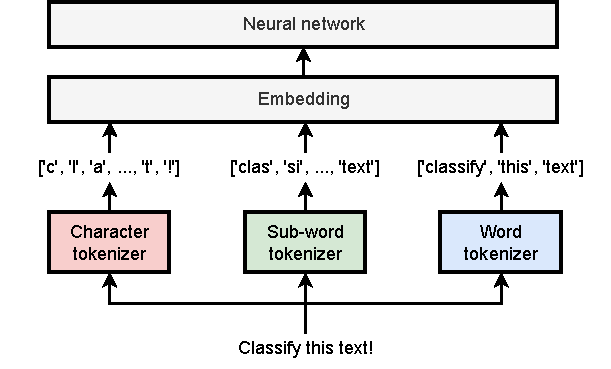
\includegraphics[width=0.7\textwidth]{images/text_tokenization}
    \caption{Начиная с текста, возможны несколько типов токенизаторов. Во всех случаях символы затем вкладываются в виде векторов и обрабатываются общей 1D-моделью.}
    \label{fig:text_tokenization}
\end{SCfigure}

Это схематически показано на Рисунке \ref{fig:text_tokenization}. Во всех трех случаях пользователь должен определить \textbf{словарь} (\textbf{вокабуляр}) допустимых токенов, например, все символы ASCII для символьного токенизатора. На практике можно выбрать желаемый размер словаря, а затем посмотреть на наиболее часто встречающиеся токены в тексте, чтобы заполнить его, при этом все остальные символы попадают в специальный токен «вне словаря» (OOV). Подсловные токенизаторы имеют для этого много специализированных алгоритмов, таких как кодирование пар байтов (BPE) \cite{shibata1999byte}.\footnote{Это краткое изложение, ориентированное на дифференцируемые модели, и мы игнорируем многие операции предварительной обработки, которые можно применять к тексту, такие как удаление стоп-слов, знаков препинания, «стемминг» и так далее. По мере роста размера моделей эти операции становятся менее распространенными.}

Поскольку большие коллекции текста могут иметь большую вариативность, предварительно обученные подсловные токенизаторы сегодня являются стандартным выбором.  В качестве конкретного примера, OpenAI выпустила версию своего собственного токенизатора с открытым исходным кодом,\footnote{\url{https://github.com/openai/tiktoken}} который является подсловной моделью, состоящей примерно из 100 тыс. подслов (на момент написания). Рассмотрим, например, кодирование «\textit{This is perplexing!}» с помощью этого токенизатора, показанное на Рисунке \ref{fig:tiktoken}. Некоторые токены соответствуют целым словам (например, «\textit{This}»), некоторые — частям слова (например, «\textit{perplex}»), а другие — знакам препинания. Последовательность можно эквивалентно представить последовательностью целых чисел:
%
\begin{equation}
[2028, 374, 74252, 287, 0]
\label{eq:list_of_indices}
\end{equation}
%
Каждое целое число находится в диапазоне от $0$ до размера словаря (в данном случае, примерно 100 тыс.) и однозначно идентифицирует токен по отношению к этому словарю. На практике ничто не мешает нам добавлять «специальные» токены в последовательность, такие как токены, представляющие начало предложения (иногда обозначаемые как [BOS]), токены OOV или что-либо еще. Токен [BOS] будет иметь особое значение в следующем разделе.

\begin{SCfigure}
    \centering
    \hspace{1em}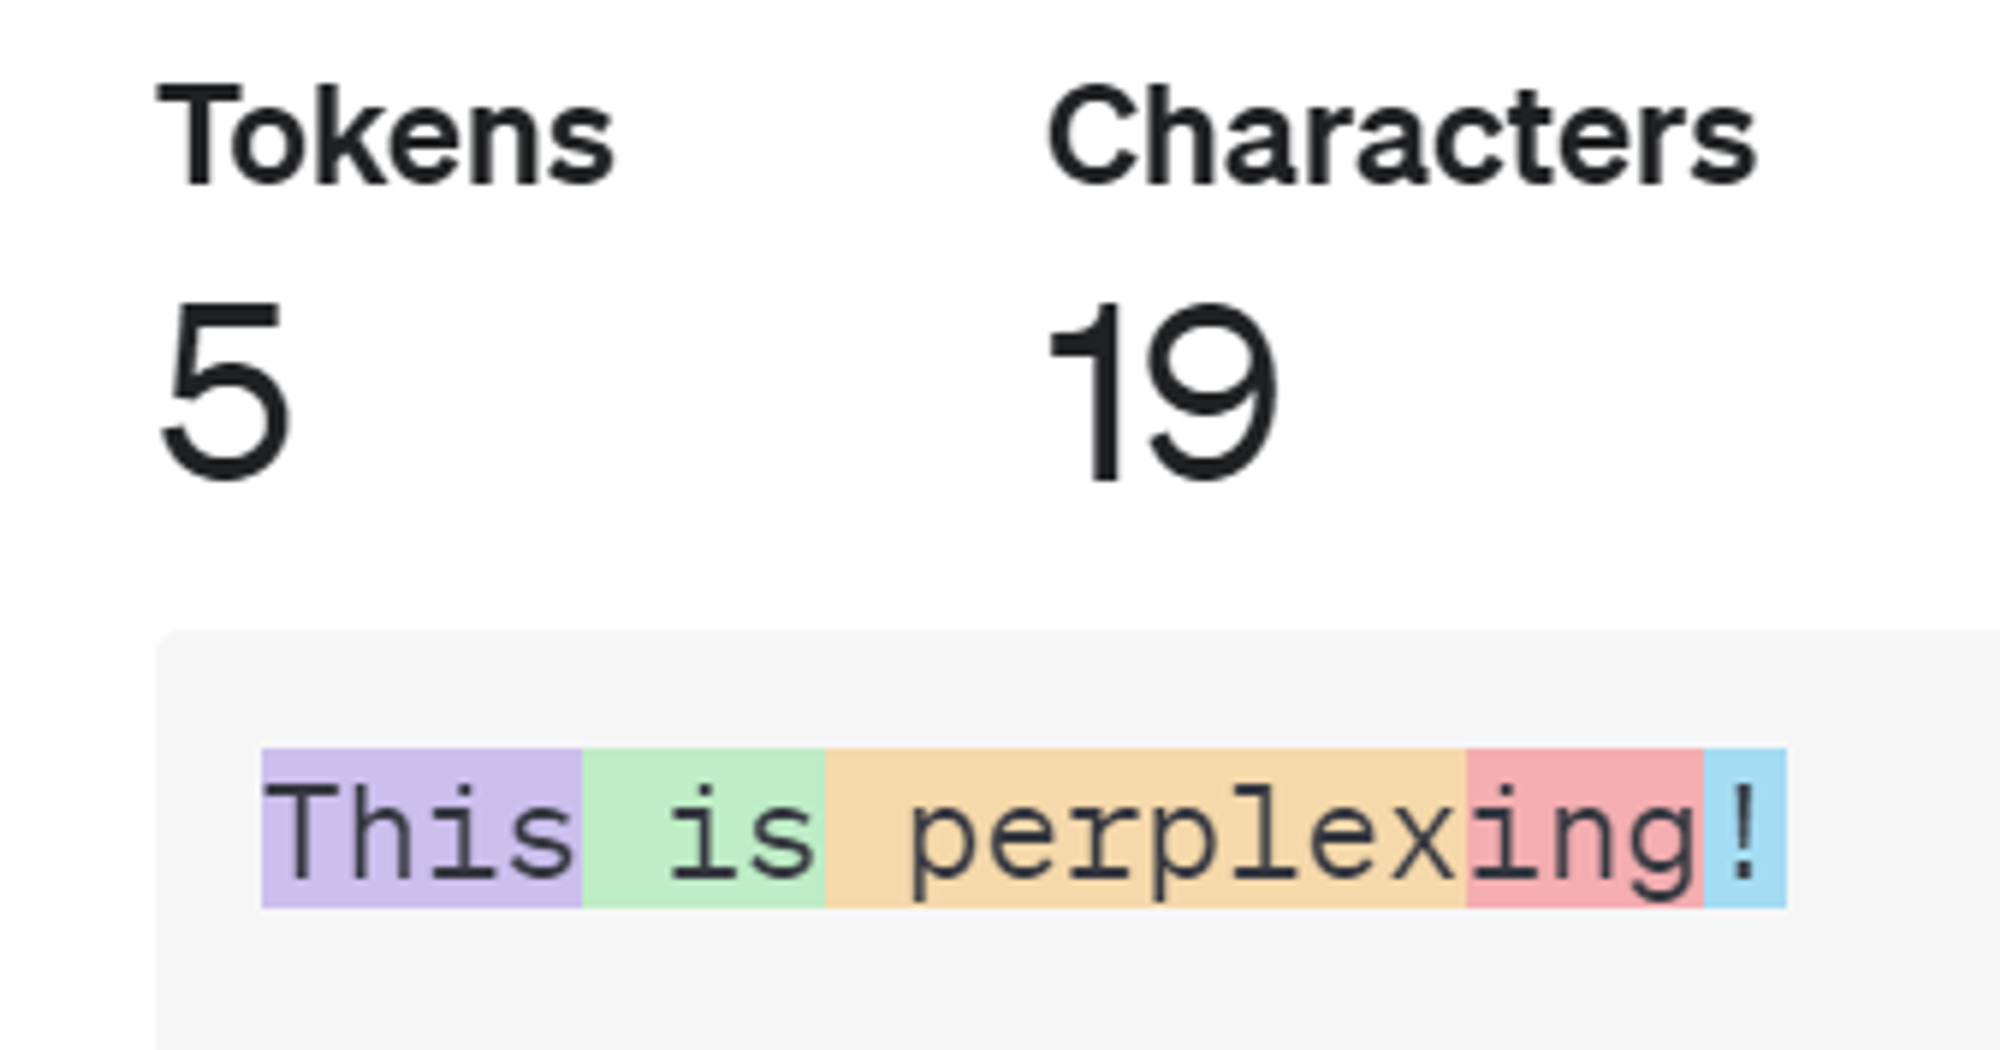
\includegraphics[width=0.35\textwidth]{images/tiktoken}
    \caption{Пример применения токенизатора tiktoken к предложению.}
    \label{fig:tiktoken}
\end{SCfigure}

Подсловная токенизация с очень большими словарями иногда может быть контринтуитивной: например, у распространенных цифр, таких как $52$, есть свой уникальный токен, в то время как цифры, такие как $2512$, могут быть разделены на токен «251» и токен «2». Для приложений, где важна обработка чисел, можно применять специализированные числовые токенизаторы \cite{golkar2023xval}. В общем, визуализация процесса токенизации всегда важна для отладки поведения моделей.

После этапа токенизации токены должны быть \textbf{вложены} в векторы, чтобы их можно было использовать в качестве входов для СНС. Простая стратегия one-hot кодирования здесь работает плохо, поскольку словари велики, и результирующие векторы будут значительно разреженными. Вместо этого у нас есть две альтернативные стратегии: первая — использовать \textit{предварительно обученные} сети, которые выполняют вложение за нас; мы рассмотрим этот вариант позже, когда будем знакомиться с трансформерами. Чтобы получить некоторое представление об этом, мы рассмотрим здесь вторую альтернативу, \textit{обучение} вложений вместе с остальной частью сети.

Предположим, мы фиксируем размерность вложения $e$ как гиперпараметр. Поскольку размер $n$ словаря также фиксирован, мы можем инициализировать матрицу вложений $\mathbf{E} \sim (n, e)$. Теперь мы определяем операцию поиска, которая заменяет каждое целое число соответствующей строкой в $\mathbf{E}$. Обозначая через $x$ последовательность идентификаторов, мы имеем:

\vspace{1em}
$$
\text{LookUp}(x) =\mathbf{X} = \begin{bmatrix}   \eqnmarkbox[drawred]{node}{\mathbf{E}_{x_1}} \\\mathbf{E}_{x_2} \\ \vdots  \\\mathbf{E}_{x_{m}}\end{bmatrix}
$$
\annotate[yshift=1em]{above,right}{node}{Строка $x_1$ в матрице вложений}

\begin{SCfigure}
    \centering
    \hspace{1em}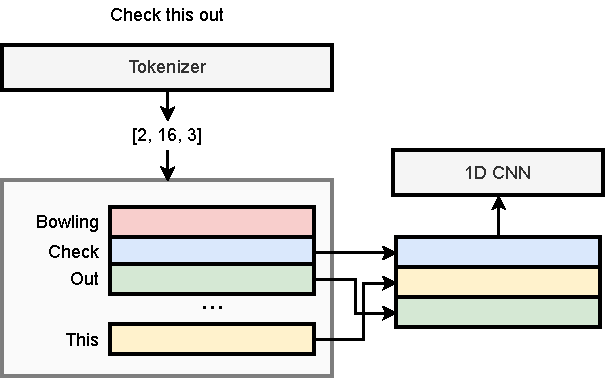
\includegraphics[width=0.6\textwidth]{images/trainable_embeddings-Page-2}
    \caption{Таблица поиска для преобразования последовательности идентификаторов токенов в их соответствующие вложения: вход — это список, выход — матрица. Вложения (показаны внутри рамки) можно обучать вместе со всеми остальными параметрами с помощью градиентного спуска. Мы предполагаем, что размер словаря равен $n=16$.}
    \label{fig:custom_embeddings}
\end{SCfigure}

\begin{mypy}{1D СНС с обучаемыми вложениями. $n$ — размер словаря, $e$ — размер каждого вложения. Мы используем два свёрточных слоя с $32$ и $64$ выходными каналами. Форма выхода для каждой операции в прямом проходе показана в виде комментария.}{code:custom_embeddings}
class TextCNN(nn.Module):
  def __init__(self, n, e):
    super().__init__()
    self.emb = nn.Embedding(n, e)
    self.conv1 = nn.Conv1d(e, 32, 5, padding='same')
    self.conv2 = nn.Conv1d(32, 64, 5, padding='same')
    self.head = nn.Linear(64, 10)

  def forward(self, x):      # (*, m)
    x = self.emb(x)          # (*, m, e)
    x = x.transpose(1, 2)    # (*, e, m)
    x = relu(self.conv1(x))  # (*, 32, m)
    x = max_pool1d(x, 2)     # (*, 32, m/2)
    x = relu(self.conv2(x))  # (*, 64, m/2)
    x = x.mean(2)            # (*, 64)
    return self.head(x)      # (*, 10)
\end{mypy}

Результирующая входная матрица $\mathbf{X}$ будет иметь форму $(m, e)$, где $m$ — длина последовательности. Теперь мы можем применить общую 1D-свёрточную модель, например, для классификации текстовой последовательности:
%
$$
\hat{y}=\text{CNN}(\mathbf{X})
$$
%
Эту модель можно обучать стандартным способом в зависимости от задачи, за исключением того, что градиентный спуск будет выполняться совместно по параметрам модели и матрице вложений $\mathbf{E}$. Это визуально показано на Рисунке \ref{fig:custom_embeddings}, а пример определения модели приведен в Листинге \ref{code:custom_embeddings}.

Эта идея чрезвычайно мощна, особенно потому, что во многих случаях мы обнаруживаем, что результирующими вложениями можно манипулировать алгебраически как векторами, например, глядя на ближайшие вложения в евклидовом смысле, чтобы найти «семантически схожие» слова или предложения. Эта идея лежит в основе использования дифференцируемых моделей во многих секторах, требующих поиска или извлечения документов.

\begin{supportbox}{Дифференцируемые модели и вложения}
Еще раз, идея вложения очень общая: любая процедура, которая преобразует объект в вектор с алгебраическими характеристиками, является вложением. Например, выход основы обученной СНС после глобального пулинга можно понимать как высокоуровневое вложение входного изображения, и его можно использовать для поиска «похожих» изображений, сравнивая его со всеми другими вложениями.
\end{supportbox}

\subsection{Работа с длинными последовательностями}

Многие из описанных ранее последовательностей могут быть очень длинными. В этом случае локальность свёрточных слоев может быть недостатком, поскольку нам нужно линейно увеличивающееся количество слоев для обработки все больших и больших рецептивных полей. В следующих главах мы увидим, что другие классы моделей (например, трансформеры) могут быть спроектированы для решения этой проблемы. Пока мы остаемся в области свёрток и покажем одно интересное решение, называемое \textbf{расширенными} (или \textbf{atrous}, от французского \textit{à trous}) свёртками, популяризированное в модели WaveNet для генерации речи \cite{oord2016wavenet}.

Мы вводим дополнительный гиперпараметр, называемый \textbf{коэффициентом расширения}. Свёртка с коэффициентом расширения $1$ — это стандартная свёртка. Для коэффициента расширения $2$ мы изменяем операцию свёртки, чтобы выбирать элементы для нашего патча, пропуская каждый второй элемент в последовательности. Аналогично, для коэффициента расширения $4$ мы пропускаем три элемента из четырех и т.д. Мы объединяем свёрточные слои с экспоненциально возрастающими коэффициентами расширения, как показано на Рисунке \ref{fig:convolution_with_dilation}.

\begin{SCfigure}
    \centering
    \hspace{1em}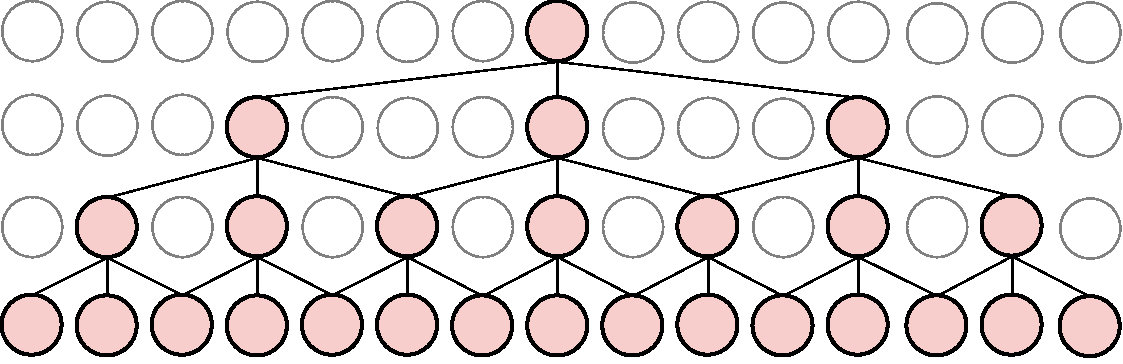
\includegraphics[width=0.55\textwidth]{images/convolution_with_dilation}
    \caption{Свёрточные слои с возрастающими коэффициентами расширения. Элементы, выбранные для свёртки, выделены красным, остальные — серым. Мы показываем рецептивное поле для одного выходного элемента.}
    \label{fig:convolution_with_dilation}
\end{SCfigure}

Количество параметров не меняется, поскольку количество соседей остается постоянным независимо от коэффициента расширения. Однако легко показать, что результирующее рецептивное поле в этом случае растет \textit{экспоненциально быстро} с числом слоев.

\section{Прогнозирование и причинные модели}
\subsection{Прогнозирование последовательностей}

Одним из важных аспектов работы с последовательностями является то, что мы можем построить модель для предсказания будущих элементов, например, цен на энергию, турбулентных потоков, загруженности колл-центров и т.д. Предсказание токенов также является фундаментальным строительным блоком для больших языковых моделей и других недавних прорывов. В очень широком смысле, большая часть нынешнего ажиотажа вокруг нейронных сетей вращается вокруг вопроса о том, насколько можно ожидать, что модель сможет делать выводы из предсказания следующего токена на больших корпусах текста, и насколько эту схему можно воспроизвести в разных модальностях (например, видео) и динамиках \cite{wang2023scientific}. Формально, предсказание следующего элемента последовательности называется \textbf{прогнозированием} в статистике и анализе временных рядов. С этого момента, чтобы соответствовать современной литературе, мы будем использовать общий термин \textbf{токен} для обозначения каждого элемента последовательности, независимо от того, имеем ли мы дело с вложенным текстовым токеном или общим векторнозначным входом.

\begin{supportbox}{Стационарность и прогнозирование}
Как и обработка текста, прогнозирование реальных временных рядов имеет ряд сопутствующих проблем (например, возможная нестационарность временного ряда, тренды и сезонность), которые мы здесь не рассматриваем.\footnote{\url{https://filippomb.github.io/python-time-series-handbook/}} На практике аудио, текст и многие другие интересующие последовательности можно считать стационарными и не требующими специальной предварительной обработки. Как и в случае с текстом, для очень больших наборов данных для прогнозирования и соответственно больших моделей влияние предварительной обработки имеет тенденцию уменьшаться \cite{ansari2024chronos}.
\end{supportbox}

Причина, по которой прогнозирование является важной проблемой, заключается в том, что мы можем обучать модель прогнозирования, имея доступ только к набору последовательностей, без необходимости в дополнительных целевых метках: в современных терминах это также называется задачей \textbf{самообучения}, поскольку цели могут быть автоматически извлечены из входов. 

Для этого предположим, что мы фиксируем заданную пользователем длину $t$ и извлекаем все возможные подпоследовательности длины $t$ из набора данных (например, при $t=12$ все последовательные окна из $12$ элементов или все предложения, состоящие из $12$ токенов и т.д.). В контексте БЯМ размер входной последовательности называется \textbf{контекстом} модели. Мы связываем с каждой подпоследовательностью целевое значение, которое является следующим элементом в самой последовательности. Таким образом, мы строим набор пар $(\mathbf{X}, \mathbf{y}), \mathbf{X} \sim (t, c) \,\, y \sim (c)$, и наша модель прогнозирования обучается с учителем на этом наборе данных:
%
$$
f(\mathbf{X})\approx \mathbf{y}
$$
%
Обратите внимание, что стандартную 1D-свёрточную модель можно использовать в качестве модели прогнозирования, обученной либо со среднеквадратичной ошибкой (для непрерывных временных рядов), либо с кросс-энтропией (для категориальных последовательностей, таких как текст). Хотя модель обучается предсказывать на один шаг вперед, мы можем легко использовать ее для генерации любого количества шагов, используя так называемый \textbf{авторегрессионный} подход, что означает, что модель предсказывает (\textit{регрессирует}) на своих собственных выходах. Предположим, мы предсказываем один шаг, $\widehat{\mathbf{y}} = f(\mathbf{X})$, и создаем «сдвинутый» вход, добавляя наше предсказанное значение к входу (удаляя первый элемент, чтобы не превышать $t$ элементов):

\begin{equation}
\mathbf{X}^\prime = \begin{bmatrix} \eqnmarkbox[drawred]{node}{\mathbf{X}_{2:t}} \\ \eqnmarkbox[drawgreen]{node2}{\widehat{\mathbf{y}}} \end{bmatrix}
\label{eq:shifted_input}
\end{equation}
\annotate[yshift=1em]{above,right}{node}{Окно из $t-1$ входных элементов}
\annotate[yshift=-1em]{below,right}{node2}{Предсказанное значение в момент времени $t+1$}

\vspace{1.5em}
\begin{supportbox}{Прогнозирование дискретных последовательностей}
Для непрерывного временного ряда это тривиально. Для временного ряда с дискретными значениями $f$ вернет вектор вероятностей по возможным значениям (т.е. возможным токенам), и мы можем получить $\widehat{\mathbf{y}}$, взяв его $\arg\max$, т.е. токен, связанный с наибольшей вероятностью. В качестве альтернативы мы можем выбрать токен пропорционально предсказанным вероятностям: см. Раздел \ref{subsec:probabilistic_formulation_generative_models}.
\end{supportbox}

Теперь мы можем запустить $f(\mathbf{X}^\prime)$, чтобы сгенерировать следующее входное значение в последовательности, и так далее итеративно, всегда обновляя наш буферизованный вход по принципу FIFO. Этот подход чрезвычайно мощен, но он требует, чтобы мы априори фиксировали длину входной последовательности, что ограничивает его применимость. Чтобы преодолеть это ограничение, нам нужна лишь незначительная модификация наших моделей.

\subsection{Причинные модели} \addclock

Предположим, у нас есть только короткая последовательность из 4 элементов, собранная в матрицу $\mathbf{X} \sim (4, c)$, но мы обучили модель прогнозирования на более длинных последовательностях с $t=6$. Чтобы запустить модель на более короткой последовательности, мы можем дополнить последовательность нулями с двумя нулевыми векторами $\mathbf{0}$ в начале, но они будут интерпретироваться моделью как фактические значения временного ряда, если мы не замаскируем ее операции. К счастью, существует более простой и элегантный подход в виде \textbf{причинных} моделей.

\begin{definition}[Причинный слой] \addbottle
Слой $\mathbf{H} = f(\mathbf{X})$ является \textbf{причинным}, если $\mathbf{H}_i = f(\mathbf{X}_{:i})$, т.е. значение, соответствующее $i$-му элементу последовательности, зависит только от элементов «из его прошлого».
\end{definition}

Модель, состоящая только из причинных слоев, конечно, сама будет причинной. Например, свёрточный слой с размером ядра $1$ является причинным, поскольку каждый элемент обрабатывается, учитывая только себя. Однако свёрточный слой с размером ядра $3$ не является причинным, поскольку он обрабатывается, учитывая дополнительно один элемент слева и один элемент справа. Мы можем преобразовать любую свёртку в причинный вариант, частично замаскировав нулями веса, соответствующие непричинным связям:
%
$$
\mathbf{h}_i=\phi\left(\left[\eqnmarkbox[drawred]{node}{\mathbf{W}\odot \mathbf{M}}\right]\text{vect}(P_{k}(i)) + \mathbf{b}\right)
$$
\annotate[yshift=-1em]{below,right}{node}{Замаскированная весовая матрица}

где $M_{ij} = 0$, если вес соответствует элементу на входе, такому что $j > i$, и $1$ в противном случае. Причинные 1D-свёртки можно комбинировать с расширенными ядрами для получения авторегрессионных моделей для аудио, как в модели WaveNet \cite{oord2016wavenet} - см. Рисунок \ref{fig:causal_convolutions} для примера.

\begin{SCfigure}
    \centering
    \hspace{1em}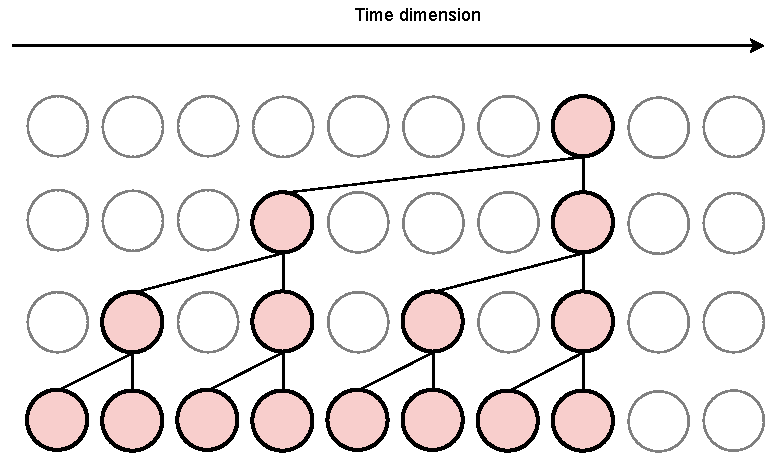
\includegraphics[width=0.5\textwidth]{images/causal_convolutions}
    \caption{Обзор 1D \textit{причинного} свёрточного слоя с (исходным) размером ядра $3$ и экспоненциально возрастающими коэффициентами расширения. Обнуленные соединения удалены, и мы показываем рецептивное поле для одного выходного элемента.}
    \label{fig:causal_convolutions}
\end{SCfigure}

Маскирование легче понять в случае одного канала, и в этом случае $\mathbf{M}$ — это просто нижнетреугольная бинарная матрица. Операция маскирования эффективно уменьшает количество параметров с $(2k+1)cc^\prime$ до $(k+1)cc^\prime$. 

Объединяя несколько причинных свёрточных слоев, мы можем получить причинный 1D-вариант модели. Предположим, мы применяем его к нашей входной последовательности, с моделью, у которой нет операций макс-пулинга. В этом случае выходная последовательность имеет ту же длину, что и входная последовательность:
%
$$
\widehat{\mathbf{Y}} = f_{\text{causal}}(\mathbf{X})
$$
%
Кроме того, любой элемент на выходе зависит только от входных элементов в той же позиции или предшествующих ей. Следовательно, мы можем определить более сложную модель прогнозирования, предсказывая значение \textit{для каждого элемента входной последовательности}. Практически, рассмотрим теперь матричный выход, определенный как:
%
$$
\mathbf{Y} = \begin{bmatrix} \mathbf{X}_{2:t} \\\mathbf{y} \end{bmatrix}
$$


\begin{figure}[t]
    \centering
    \begin{subfigure}[b]{0.45\textwidth}
    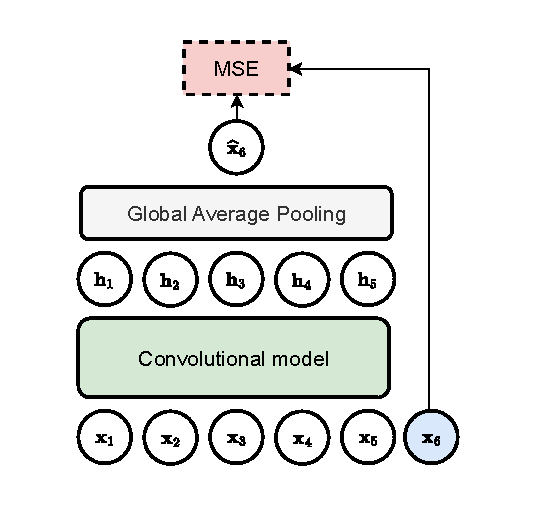
\includegraphics[width=1.0\textwidth]{images/forecasting-Page-1}
    \caption{Непричинная модель}
    \label{fig:forecasting_a}
    \end{subfigure}
    \begin{subfigure}[b]{0.48\textwidth}
    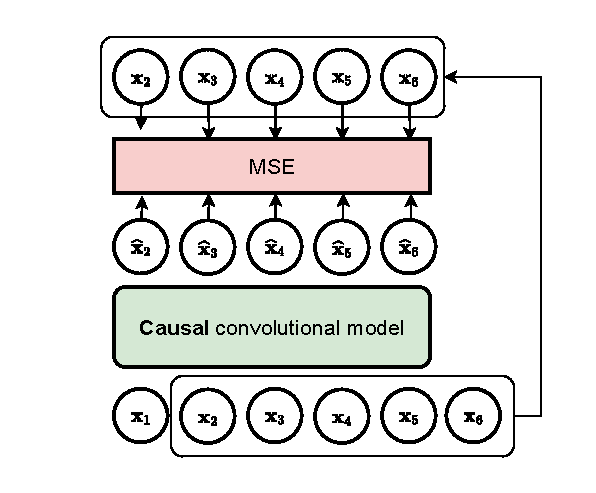
\includegraphics[width=1.0\textwidth]{images/forecasting-Pagina-2}
    \caption{Причинная модель}
    \label{fig:forecasting_b}
    \end{subfigure}
    \caption{Сравнение между (a) непричинной моделью для прогнозирования (предсказывающей только один элемент для всей входной последовательности) и (b) причинной моделью, обученной предсказывать один выходной элемент для каждого входного элемента в последовательности.}
    \label{fig:forecasting}
\end{figure}


Это похоже на сдвинутый вход из \eqref{eq:shifted_input}, за исключением того, что мы добавляем истинное значение в качестве последнего элемента последовательности. Мы можем обучать эту модель, минимизируя потери по всем элементам, например, среднеквадратичную ошибку:
%
\begin{equation}
l(\widehat{\mathbf{Y}},\mathbf{Y})=\lVert \widehat{\mathbf{Y}} - \mathbf{Y} \rVert^2=\sum_{i=1}^t \eqnmarkbox[drawred]{node}{\lVert \widehat{\mathbf{Y}}_i - \mathbf{Y}_i \rVert^2}
\label{eq:mse_forecasting_multiple}
\end{equation}
\annotate[yshift=-1em]{below,right}{node}{Потери при предсказании $\mathbf{X}_{i+1}$}

Мы одновременно предсказываем второй элемент на основе первого, третий — на основе первых двух и т.д. Для одного входного окна у нас есть $t$ отдельных членов потерь, что значительно улучшает распространение градиента. Сравнение двух подходов показано на Рисунке \ref{fig:forecasting}: на Рисунке \ref{fig:forecasting_a} мы показываем непричинную свёрточную модель, обученную предсказывать следующий элемент в последовательности, а на Рисунке \ref{fig:forecasting_b} — причинную модель, обученную в соответствии с \eqref{eq:mse_forecasting_multiple}.

\begin{figure}
    \centering
    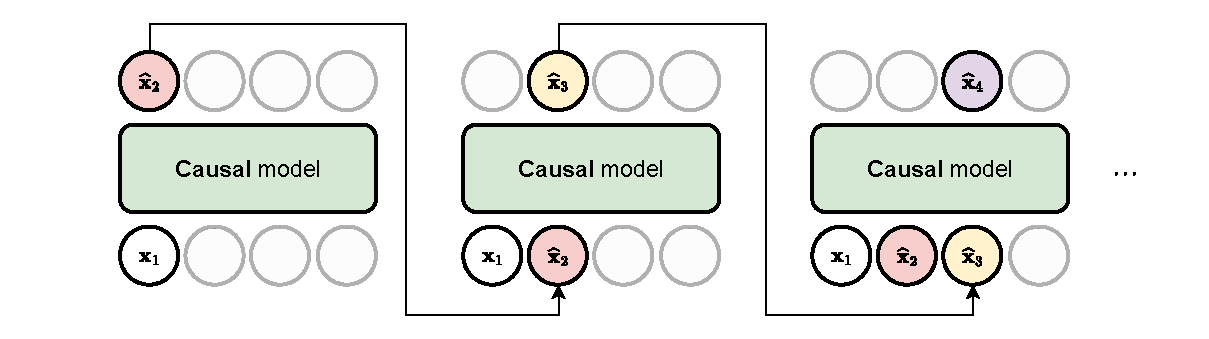
\includegraphics[width=0.95\textwidth]{images/forecasting-Pagina-3}
    \caption{Вывод с помощью причинной СНС, генерирующей последовательность шаг за шагом авторегрессионным способом. Неиспользуемые входные токены затенены. Сгенерированные токены окрашены в разные цвета для их различения.}
    \label{fig:forecasting_autoregressive}
\end{figure}

Что еще более важно, теперь мы можем использовать модель авторегрессионным способом с любой длиной последовательности до максимальной длины $t$. Это легко увидеть на примере. Предположим, у нас $t=4$, и мы наблюдали два значения $\mathbf{x}_1$ и $\mathbf{x}_2$. Мы вызываем модель в первый раз, дополняя последовательность нулями, чтобы сгенерировать третий токен:
%
$$
\begin{bmatrix} - \\  {\color{drawred}\widehat{\mathbf{x}}_3} \\ - \\ - \end{bmatrix} =f\left( \begin{bmatrix} \mathbf{x}_1 \\ \mathbf{x}_2 \\ \mathbf{0} \\ \mathbf{0} \end{bmatrix} \right)
$$
%
Мы игнорируем все выходные значения, кроме второго (фактически, третье и четвертое выходы недействительны из-за дополнения нулями). Мы добавляем $\widehat{\mathbf{x}}_3$ к последовательности и продолжаем вызывать модель авторегрессионно (мы показываем предсказанные значения цветом):



$$
\begin{bmatrix} - \\  - \\ {\color{drawgreen}\widehat{\mathbf{x}}_4} \\ - \end{bmatrix} =f\left( \begin{bmatrix} \mathbf{x}_1 \\ \mathbf{x}_2 \\ {\color{drawred}\widehat{\mathbf{x}}_3} \\ \mathbf{0} \end{bmatrix} \right) \;,\;\begin{bmatrix} - \\  - \\ - \\ {\color{drawblue}\widehat{\mathbf{x}}_5} \end{bmatrix} =f\left( \begin{bmatrix} \mathbf{x}_1 \\ \mathbf{x}_2 \\ {\color{drawred}\widehat{\mathbf{x}}_3} \\ {\color{drawgreen}\widehat{\mathbf{x}}_4} \end{bmatrix} \right) \;,\; \begin{bmatrix}  - \\ - \\ - \\{\color{orange}\widehat{\mathbf{x}}_6}  \end{bmatrix} =f\left( \begin{bmatrix} \mathbf{x}_2 \\ {\color{drawred}\widehat{\mathbf{x}}_3} \\ {\color{drawgreen}\widehat{\mathbf{x}}_4} \\ {\color{drawblue}\widehat{\mathbf{x}}_5} \end{bmatrix}  \right) \; \ldots
$$

На последнем шаге мы удалили один из исходных входов, чтобы сохранить ограничение на размер входа. Это также показано на Рисунке \ref{fig:forecasting_autoregressive}. Обратите внимание, что модель обучается только на реальных значениях, а не на своих собственных предсказаниях: это называется \textbf{обучением с учителем}. Вариант обучения с учителем заключается в постепенной замене некоторых значений в мини-пакетах значениями, предсказанными моделью, по мере того как обучение продолжается и модель становится более точной. 

Причинные авторегрессионные модели особенно интересны в случае текстовых последовательностей (где у нас есть только один канал, индекс токенов), поскольку мы можем начать с одного токена [BOS], представляющего начало последовательности, и генерировать текстовые предложения с нуля, или \textit{обусловливать} генерацию конкретным запросом пользователя, который добавляется к токену [BOS]. Аналогичное рассуждение можно применить к аудиомоделям для генерации речи или музыки \cite{oord2016wavenet}.

\section{Авторегрессионные и генеративные модели}
\subsection{Вероятностная формулировка генеративных моделей}
\label{subsec:probabilistic_formulation_generative_models} \addteacup

Авторегрессионная модель — это простой пример \textbf{генеративной модели}.\footnote{Напомним из Главы \ref{chap:supervised_learning}, что мы предполагаем, что наши пары для обучения с учителем $(x,y)$ происходят из некоторого неизвестного распределения вероятностей $p(x,y)$. По правилу произведения вероятностей мы можем разложить его эквивалентно как $p(y \mid x)p(x)$ или $p(x \mid y)p(y)$. Любая модель, которая аппроксимирует $p(x)$ или $p(x \mid y)$, называется \textbf{генеративной}, потому что вы можете использовать ее для выборки новых входных точек. Напротив, модель, которая аппроксимирует только $p(y \mid x)$, как мы делали в предыдущих главах, называется \textbf{дискриминативной}.} Мы подробно поговорим о других типах генеративных моделей в следующем томе. Пока мы приводим некоторые идеи, специфичные для авторегрессионных алгоритмов. Мы рассматриваем последовательности с одним каналом и дискретными значениями, такие как текст. Авторегрессионные модели над текстовыми токенами являются основой БЯМ и могут использоваться в качестве основы для мультимодальных архитектур (Глава \ref{chap:transformers_in_practice}).

Генеративные модели более естественно формулируются в контексте вероятностей, поэтому мы начнем с переформулировки нашего предыдущего обсуждения с помощью вероятностного формализма. Обозначим через $\mathcal{X}$ пространство всех возможных последовательностей (например, все возможные комбинации текстовых токенов). В общем, многие из этих последовательностей будут недействительными, например, последовательность [«\textit{тт}», «\textit{тт}»] на английском языке. Однако даже очень редкие последовательности могут встречаться хотя бы один или два раза в очень больших корпусах текста (представьте себе персонажа, кричащего «\textit{Скотттт!}»). 

Мы можем обобщить это, рассмотрев распределение вероятностей $p(x)$ по всем возможным последовательностям $x \in \mathcal{X}$. В контексте текста это также называется \textbf{языковой моделью}. Генеративное моделирование — это задача научиться эффективно выбирать из этого распределения:\footnote{В этом разделе $\sim$ используется для обозначения выборки из распределения вероятностей, а не формы тензора.}
%
$$
x \sim p(x)
$$
%
Чтобы увидеть, как это связано с нашим предыдущим обсуждением, обратите внимание, что по правилу произведения вероятностей мы всегда можем переписать $p(x)$ как:
%
\begin{equation}
p(x)=\prod_ip(x_i \mid x_{:i})
\label{eq:prob_autoregressive}
\end{equation}
%
где мы обусловливаем каждое значение $x_i$ всеми предшествующими значениями. Если мы предположим, что длина входа нашей модели достаточно велика, чтобы вместить все возможные последовательности, мы можем использовать причинную модель прогнозирования для параметризации распределения вероятностей в \eqref{eq:prob_autoregressive}:
%
$$
p(x_i \mid x_{:i})=\text{Categorical}(x_i\mid f(x_{:i}))
$$
%
где мы используем одну, общую модель для всех временных шагов. Максимальное правдоподобие для этой модели тогда эквивалентно минимизации кросс-энтропийной потери по предсказанным вероятностям, как в Разделе \ref{subsec:logistic_regression}.

\subsection{Выборка в авторегрессионной модели}

В общем, выборка из распределения вероятностей нетривиальна. Однако для авторегрессионных моделей мы можем использовать разложение произведения в \eqref{eq:prob_autoregressive} для разработки простой итерационной стратегии:
%
\begin{enumerate}
\item Выбрать $x_1 \sim p(x_1)$. Это эквивалентно обусловливанию на пустом множестве $p(x_1 \mid \{\})$. На практике мы всегда обусловливаем на начальном фиксированном токене, таком как токен [BOS], чтобы наш вход никогда не был пустым.
\item Выбрать $x_2 \sim p(x_2 \mid x_1)$, снова запустив сеть со значением, которое мы выбрали на шаге (1), как на Рисунке \ref{fig:forecasting_autoregressive}.
\item Выбрать $x_3 \sim p(x_3 \mid x_1, x_2)$.
\item Продолжать до тех пор, пока мы не достигнем желаемой длины последовательности или пока не получим токен конца предложения.
\end{enumerate}

Мы делали это неявно ранее, всегда выбирая элемент с наибольшей вероятностью:
%
$$
x_i=\underset{i}{\arg\max} \;f(x_{:i})
$$
%
Однако мы также можем обобщить это, выбирая значение в соответствии с вероятностями, предсказанными $f$. Помните (Раздел \ref{sec:softmax}), что softmax можно обобщить, рассмотрев дополнительный параметр температуры. Изменяя этот параметр во время вывода, мы можем плавно переходить от всегда выбора значения argmax (очень низкая температура) до почти равномерного распределения по токенам (очень высокая температура).

В контексте вероятностного моделирования выборка таким образом из этого класса моделей называется \textbf{выборкой по предкам}, в то время как в контексте языкового моделирования мы иногда используем термин \textbf{жадное декодирование}. Использование термина «жадный» и это краткое обсуждение достаточно, чтобы подчеркнуть один потенциальный недостаток этих моделей: хотя разложение произведения $p(x)$ является точным, жадное декодирование не гарантирует получение выборки, соответствующей высоким значениям $p(x)$. 

Чтобы увидеть это, обратите внимание, что $f$ дает оценку вероятности для одного токена, но вероятность последовательности задается произведением многих таких членов. Следовательно, выборка токена с высокой (локальной) вероятностью в начале последовательности может не соответствовать последовательности, имеющей большую (глобальную) вероятность как предложение. Это легко представить, если вы представите, что выбор первого токена заставляет этап декодирования «застревать» на пути с низкой вероятностью.

Распространенным смягчением этой проблемы является \textbf{лучевой поиск} (или \textbf{лучевое декодирование}). При лучевом поиске на первом шаге мы выбираем $k$ различных элементов (называемых лучами, где $k$ — заданный пользователем параметр). На втором шаге для каждого из наших $k$ лучей мы выбираем $k$ возможных продолжений. Из этих $k^2$ пар мы сохраняем только $k$ лучших значений с точки зрения их произведения вероятностей $p(x_1)p(x_2\mid x_1)$ (или, что эквивалентно, их логарифма вероятности). Мы продолжаем итеративно таким образом до конца последовательности.

Рассматривая с этой точки зрения, выборка наиболее вероятной последовательности из нашей авторегрессионной модели — это комбинаторная задача поиска (представьте себе дерево, где для каждого токена мы расширяемся по всем возможным следующим токенам и так далее). С точки зрения компьютерного программирования, лучевой поиск тогда является примером \textbf{поиска в ширину} по этому дереву.

\subsection{Условное моделирование}
\label{subsec:conditional_modelling}

Как мы уже упоминали ранее, в общем случае нас может интересовать не столько генерация последовательностей с нуля, сколько генерация продолжений известных последовательностей, таких как вопрос или взаимодействие пользователя. Это можно формализовать, рассмотрев \textit{условные} распределения вероятностей в форме $p(x \mid c)$, где $c$ — это условный аргумент, такой как запрос пользователя. Наше предыдущее обсуждение почти прямолинейно распространяется на этот случай. Например, разложение произведения теперь записывается как:
%
$$
p(x \mid c)=\prod_ip(x_i \mid x_{:i},c)
$$
%
где мы обусловливаем на предыдущих входах \textit{и} контексте пользователя. Выборка, декодирование и т.д. расширяются аналогичным образом. 

Для выполнения условной генерации мы параметризуем $p(x_i \mid x_{:i},c)$ нейронной сетью $f(x,c)$ так, что:
%
$$
p(x_i \mid x_{:i},c) \approx \text{Categorical}(x_i \mid f(x_{:i}, c))
$$
%
Следовательно, основное отличие от безусловного случая заключается в том, что нам нужна функция $f(x,c)$, имеющая два входных аргумента и удовлетворяющая причинности по первому аргументу. При работе с авторегрессионными моделями, если и $x$, и $c$ являются текстами, мы можем легко сделать это, рассматривая $c$ как часть входной последовательности и работая с одной объединенной входной последовательностью $x^\prime = [c \Vert x]$. Например, с запросом пользователя «\textit{Столица Франции}», для простоты взяв словный токенизатор, мы могли бы иметь:\footnote{Мы игнорируем наличие токена конца последовательности (EOS) для остановки авторегрессионной генерации.}
%
$$
f_{\text{causal}}([\text{Столица}, \text{Франции}]) = {\color{drawred}\text{—}} \\
f_{\text{causal}}([\text{Столица}, \text{Франции}, {\color{drawred}\text{—}}]) = {\color{drawgreen}\text{Париж}} \\
$$
%
Следовательно, мы можем обрабатывать безусловное и условное моделирование одновременно с помощью одной модели.\footnote{Мы увидим в Главе \ref{chap:transformers_in_practice}, что почти любой тип данных можно преобразовать в последовательность токенов. Предположим, мы генерируем текстовую последовательность, обусловленную изображением (например, \textbf{создание подписей к изображениям}). Если и текст, и изображения преобразуются в токены с одинаковым размером вложения, мы можем применить авторегрессионную модель, объединив токены из двух типов входа (также называемых \textbf{модальностями} в этом контексте), где мы рассматриваем токены изображения как условное множество $c$.}
 В следующем томе мы увидим другие примеры условных генеративных моделей, в которых необходимы более сложные стратегии. Мы также расширим эту тему, когда будем обсуждать модели-декодеры трансформеров в Главе \ref{chap:transformers_in_practice}.

\section*{От теории к практике}

\begin{wrapfigure}{r}{3.0cm}
\vspace{-3em}
\includegraphics[width=3.0cm]{images/shutterstock_2075221579.jpg}
\vspace{-2em}
\end{wrapfigure}

Работа с текстовыми данными сложнее, чем классификация изображений, из-за многих тонкостей, связанных с токенизацией, форматированием данных, странными символами и последовательностями переменной длины. У PyTorch есть своя текстовая библиотека, \texttt{torchtext}, которая на момент написания менее документирована, чем основная библиотека, и полагается на другую бета-библиотеку (\texttt{torchdata}) для обработки конвейеров данных. Поэтому мы здесь ее игнорируем, но приглашаем вас ознакомиться с ней самостоятельно.

Hugging Face Datasets, вероятно, является самым универсальным инструментом в этом случае, поскольку он предоставляет обширный массив наборов данных и предварительно обученных токенизаторов, которые можно немедленно экспортировать в PyTorch.\footnote{См. это руководство для получения инструкций: \url{https://huggingface.co/docs/datasets/use_dataset}.} Ознакомьтесь немного с библиотекой, прежде чем приступать к упражнению.

\begin{enumerate}
\item Выберите набор данных для классификации текста, например, классический набор данных IMDB.\footnote{\url{https://huggingface.co/datasets/stanfordnlp/imdb}} 
\item Токенизируйте его, чтобы получить набор данных вида $(x,y)$, где $x$ — это список целых чисел, как в \eqref{eq:list_of_indices}, а $y$ — текстовая метка.
\item Постройте и обучите 1D-свёрточную модель, похожую на Листинг \ref{code:custom_embeddings}. Немного поэкспериментируйте с дизайном модели, чтобы увидеть ее влияние на конечную точность.
\end{enumerate}

В PyTorch нет быстрого способа сделать 1D-свёртку причинной, поэтому мы отложим наши авторегрессионные эксперименты до тех пор, пока не представим трансформеры.\footnote{Если вы хотите попробовать, вы можете эмулировать причинную свёртку с правильным дополнением; см. Лекцию 10.2 здесь: \url{https://fleuret.org/dlc/}. Весь курс действительно хорош, если вы ищете потоковые лекции.} Обучение собственного токенизатора — очень хорошее дидактическое упражнение, хотя оно далеко выходит за рамки этой книги. Для введения вы можете ознакомиться с этой минималистичной реализацией BPE: \url{https://github.com/karpathy/minbpe}.